\begin{frame}{Preliminaries}
    Fixed a graph $G = (V, E)$ where $V = \{v_1, \dots, v_n\}$
    \pause
    \bigbreak
    \begin{enumerate}[-]
        \item A \emph{cut list} is a list of pairs $\call = \{(S_1, \ell_1), \dots, (S_m, \ell_m)\}$;
        
        \item For each $j$ we have $\emptyset \ne S_j \subsetneq V$ and $\ell_j \in \N$;
        
        \item $G$ \emph{realizes} $\mathcal{L}$ if $|\partial(S_j)|=\ell_j$ for every $(S_j, \ell_j) \in \mathcal{L}$;

        \item By $w(\call)$ we denote $\max_j\ |S_j|$.
    \end{enumerate}
\end{frame}

\begin{frame}{New Graph Realization Problem}
  \defproblema{Graph Realization with Cut Constraints (GR-C)}
    {A cut list $\call$ for a set of vertices $V = \{v_1, \dots, v_n\}$, and a non-decreasing sequence $\texttt{d} = (d_1, \dots, d_n)$ of natural numbers.}
    {Does there exist a simple graph $G = (V, E)$ such that, for every $j$, $d(v_j) = d_j$ and $G$ realizes $\call$?}
\end{frame}

\begin{frame}{Running Example}
  \centering
  Consider $\texttt{d}=(3, 2, 2, 2, 1)$ and $\call = \{(\{a, d\}, 4), (\{c, d, e\}, 2)\}:$
  \pause
  \bigbreak
  \begin{minipage}{\linewidth}
    \centering
    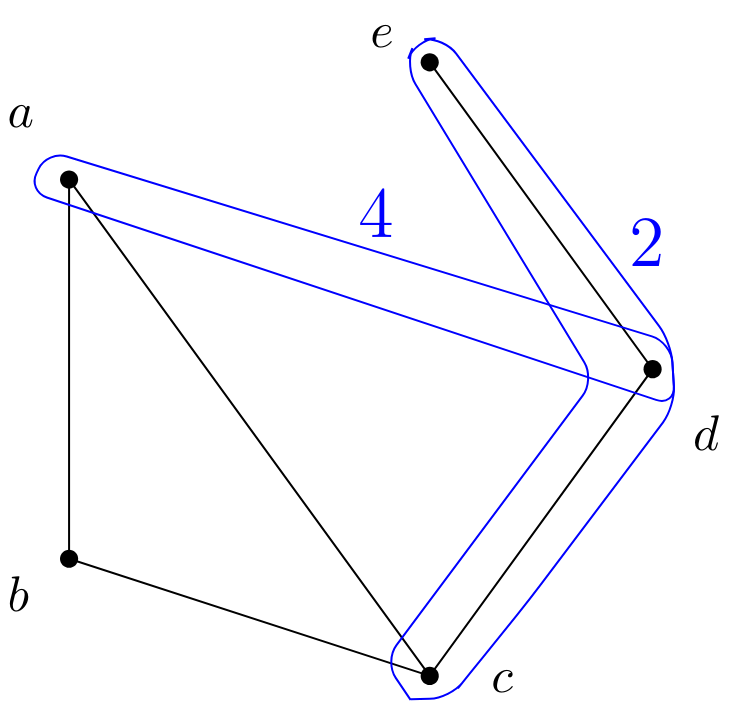
\includegraphics[height=4cm]{images/cut1.png}
    \pause
    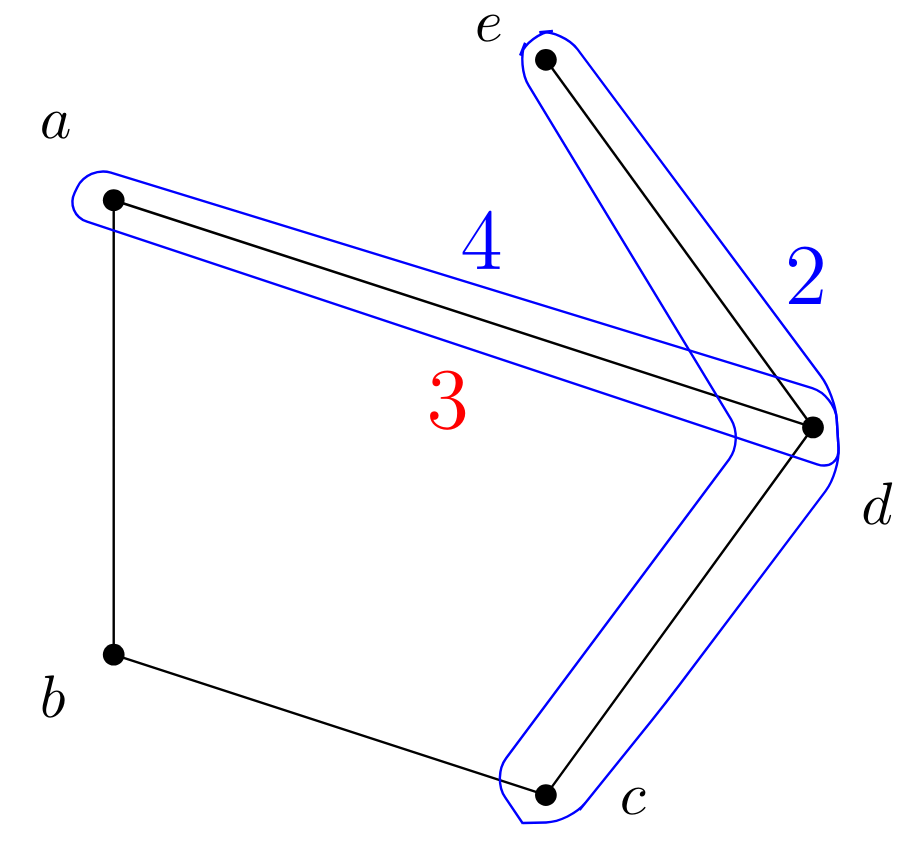
\includegraphics[height=4cm]{images/cut2.png}
  \end{minipage}
\end{frame}

\begin{frame}{Observations}
    \begin{enumerate}[-]

    \item If $\call = \emptyset$, we have the classic realization problem;

    % \item Assume that $2 \le |S_j| \le n-2$ for every $j$;

    \item We can see GR-C as a consistency check for cut-queries in learning an unknown graph.

  \end{enumerate}
\end{frame}

\begin{frame}{Important Remark}
    \centering
    For $S \subseteq V$ let $d(S) = \sum\limits_{u \in S} d(u)$.
    \bigbreak
    \pause
    \begin{remark}[1]
        An instance $(\texttt{d}, \call)$ is true only if, for each $(S, \ell) \in \call$, $\ell \in \{ d(S) - 2k \mid 0 \leq k \leq \binom{|S|}{2} \}$.
    \end{remark}
\end{frame}

\subsection{Small Cuts}

\begin{frame}{Fixed Edges}
    For a solution $G$ if $(\set{u, v}, d(u) + d(v) - 2) \in \call$ then $uv \in E(G)$.
\end{frame}

\begin{frame}{Forbidden Edges}
    For a solution $G$ if $(\set{u, v}, d(u) + d(v)) \in \call$ then $uv \notin E(G)$.
\end{frame}

\begin{frame}{Simplification}
    Replace $(\set{u, v}, d(u) + d(v) - 2)$ by $(\set{u, v}, d(u) + d(v))$ while updating $\texttt{d}$.
\end{frame}

\begin{frame}{Possibility Graph}
    \centering
    Let $F$ be the set of forbidden edges.
    \pause
    \bigbreak
    Then we call $\calg = K_n - F$ the \emph{possibility graph}.
\end{frame}

\begin{frame}{Size 2 Cut Constraints}
    \centering
    We can reduce GR-C to $f$-factor!
    \pause
    \bigbreak
    \begin{lemma}[1]
        An instance $(\texttt{d}, \call)$ of GR-C can be solved in polynomial time whenever $w(\call) = 2$.
    \end{lemma}
\end{frame}

\begin{frame}{Size 3 Cut Constraints}
    \centering
    We can reduce to the previous case!
    \pause
    \bigbreak
    \begin{theorem}[1]
        An instance $(\texttt{d}, \call)$ of GR-C can be solved in polynomial time whenever $w(\call) = 3$.
    \end{theorem}
\end{frame}

\begin{frame}{Proof}
    \centering
    Consider a cut $(S, \ell) \in \call$ where $S = \set{u, v, w}$.
\end{frame}

\begin{frame}{Case $\ell = d(S)$}
    \centering
    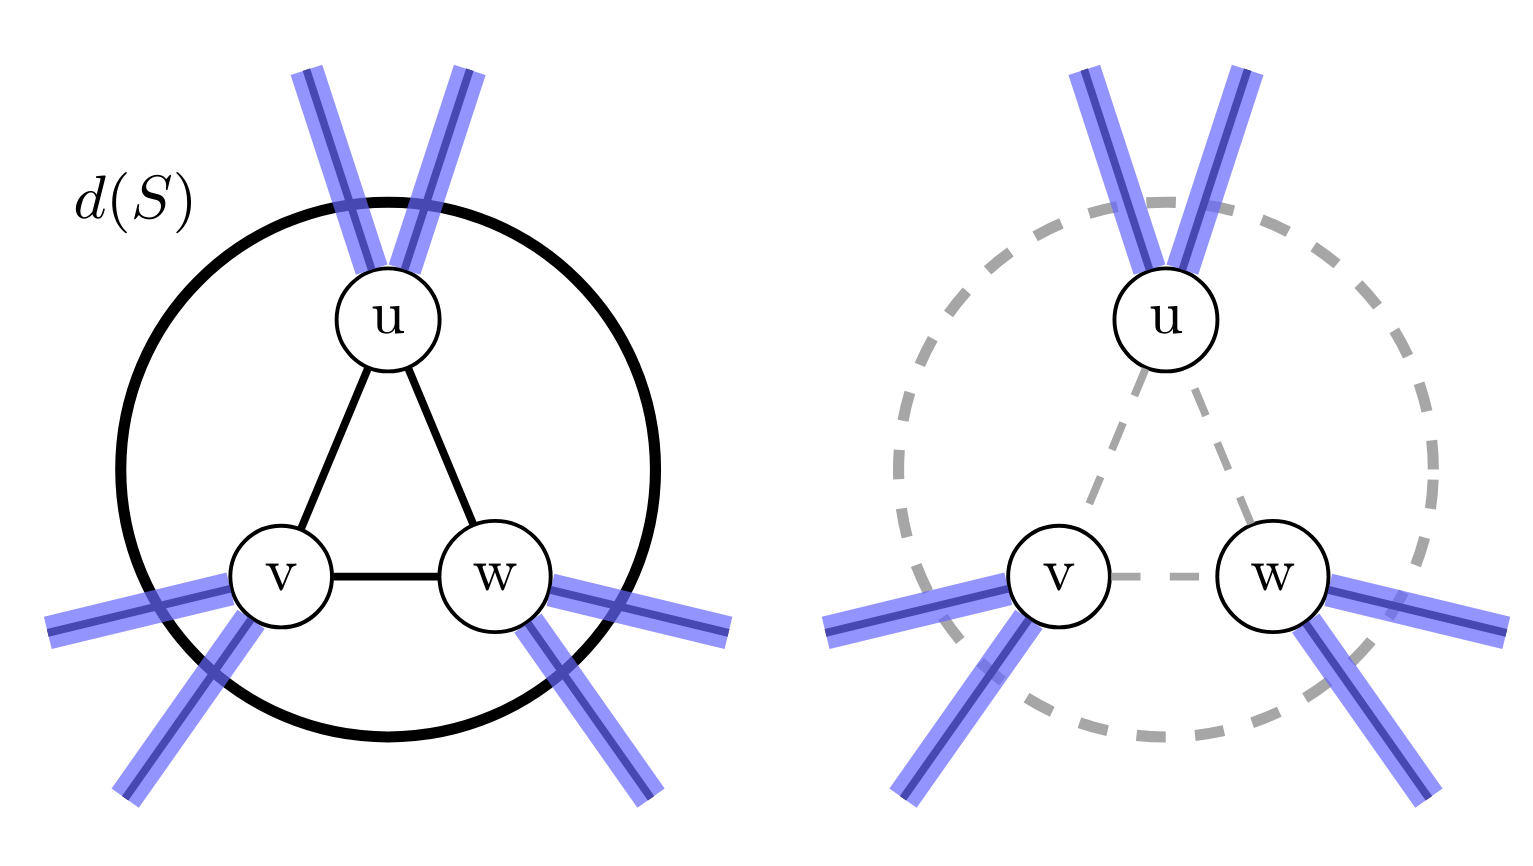
\includegraphics[height=4cm]{images/3cut1.png}
\end{frame}

\begin{frame}{Case $\ell = d(S) - 4$}
    \centering
    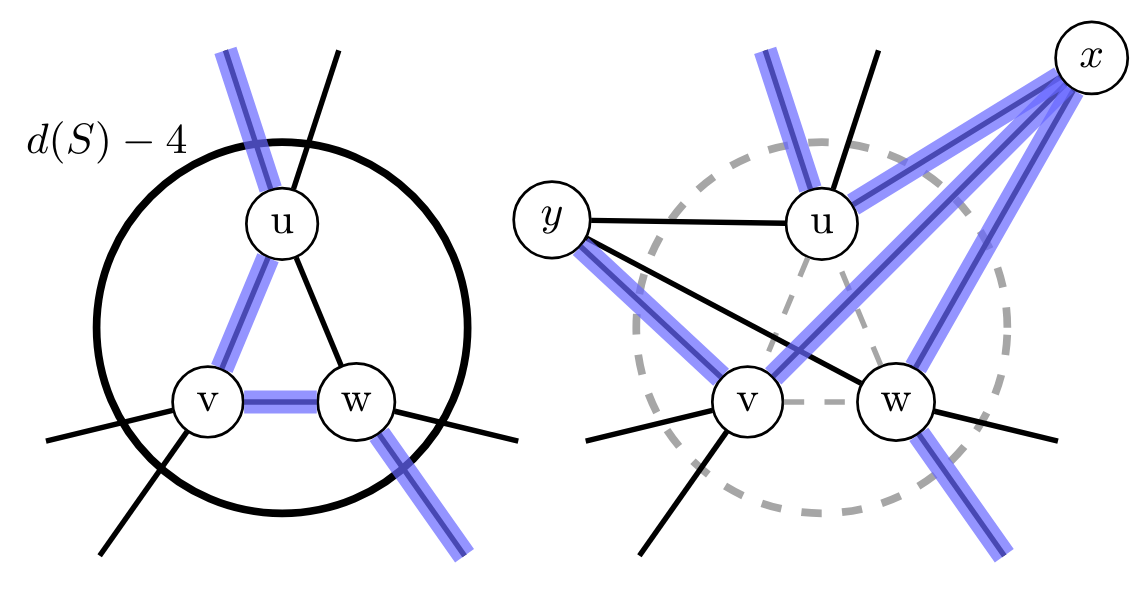
\includegraphics[height=4cm]{images/3cut4.png}
\end{frame}

\begin{frame}{Other Cases}
    \centering
    \Large
    $\ell = d(S) - 2$ or $\ell = d(S) - 6$
\end{frame}

\begin{frame}{Running Example}
  \centering
  $\texttt{d}=(3, 2, 2, 2, 1)$ and $\call = \{(\{a, d\}, 4), (\{c, d, e\}, 2)\}$:
  \bigbreak
  \begin{minipage}{\linewidth}
    \centering
    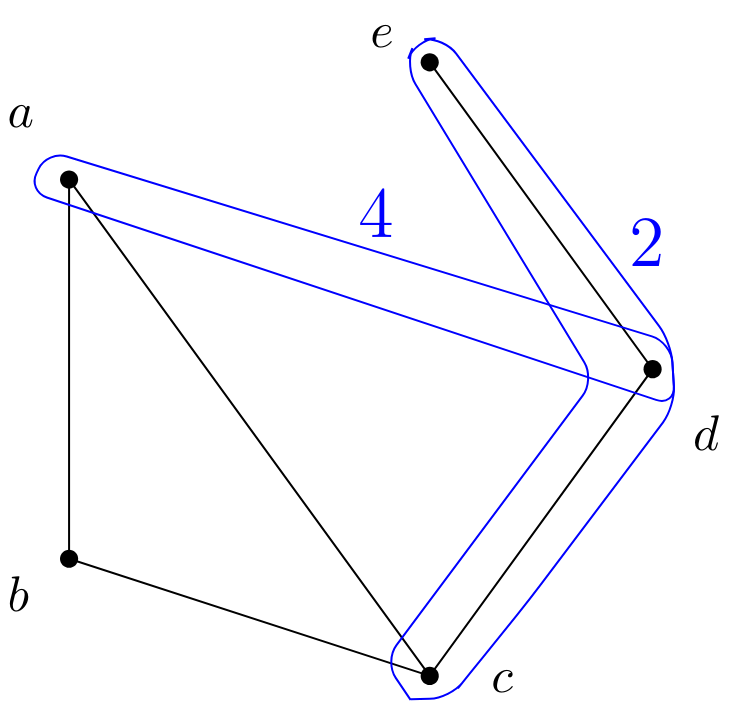
\includegraphics[height=6cm]{images/cut1.png}
  \end{minipage}
\end{frame}

\begin{frame}{Running Example}
  \centering
  Equivalent $f$-factor instance:
  \bigbreak
  \begin{minipage}{\linewidth}
    \centering
    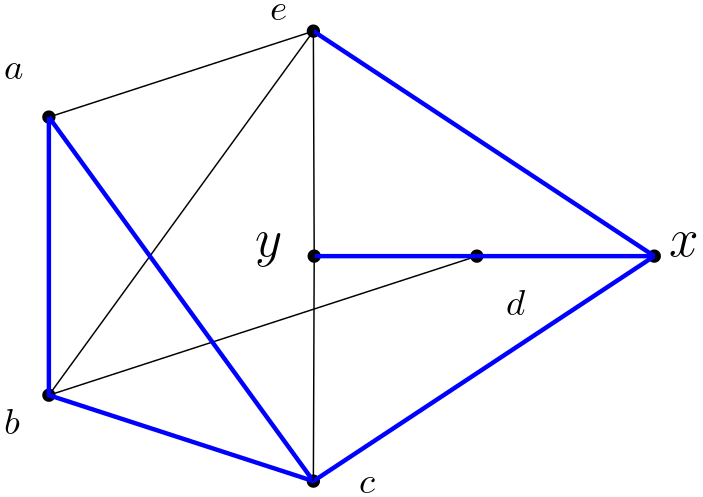
\includegraphics[height=4cm]{images/factor1.png}
  \end{minipage}
\end{frame}

\subsection{Large Cuts}

\begin{frame}{Size 4 Cut Constraints}
    \centering
    Can we keep doing a case-by-case analysis?
    \pause
    \bigbreak
    No, we cannot, as the GR-C becomes hard!
\end{frame}

\begin{frame}{Intuition}
    \centering
    For $S \in \binom{V}{3}$, the edges within $S$ determine how degrees change.
    \pause
    \bigbreak
    In contrast, when $S \in \binom{V}{4}$, this claim does not hold anymore.
\end{frame}

\begin{frame}{Hardness}
    \centering
    \begin{theorem}[2]
        The GR-C problem cannot be solved in polynomial time unless $P = NP$ even when $w(\call) = 4$ and all degrees in the degree sequence $\texttt{d}$ are 1.
    \end{theorem}
\end{frame}

\begin{frame}{Proof}
    \centering
    Reduction from $k$-True \rXthreeSAT{}
\end{frame}

\begin{frame}{\rXthreeSAT{}}
    \beamerdefaultoverlayspecification{}
    \defproblema{\rXthreeSAT{}}{
        A set of variables $X$ and a formula~$\phi$ in conjunctive normal form over $X$ such that:
        \begin{itemize}
            \item each variable of $X$ occurs twice as a positive literal and once as a negative literal;
            \item each clause of $\phi$ has two or three literals.
        \end{itemize}
    }{Is there a truth assignment of $X$ such that exactly one literal in every clause of $\phi$ is true?}
\end{frame}

\begin{frame}{\rXthreeSAT{}}
    \begin{lemma}[2]
        \rXthreeSAT{} is NP-complete.
    \end{lemma}
\end{frame}

\begin{frame}{\kXthreeSAT{}}
    \defproblema{\kXthreeSAT{}}{
        A tuple $(X, \phi, k)$, where $(X, \phi)$ is an instance of \rXthreeSAT{} and $k$ is a nonnegative integer.
    }{Is there a feasible solution to $(X, \phi)$ in which exactly $k$ variables are assigned to true?}
\end{frame}

\begin{frame}{\kXthreeSAT{}}
    \begin{lemma}[3]
        \kXthreeSAT{} cannot be solved in polynomial time unless $P = NP$.
    \end{lemma}
\end{frame}

\begin{frame}{Variable Gadget}
    \begin{minipage}{\linewidth}
        \centering
        \only<1>{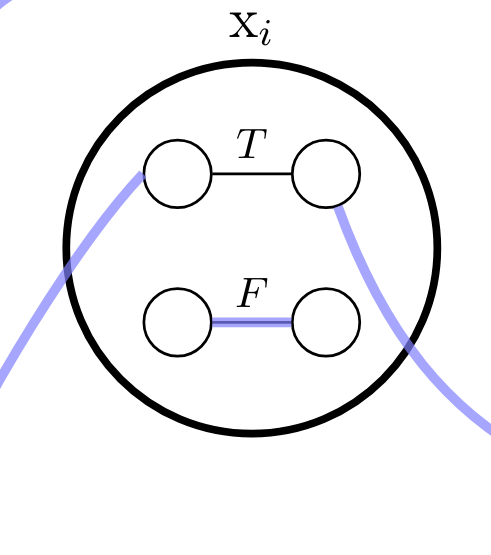
\includegraphics[clip, trim={0 0 0 0.2cm}, height=4.7cm]{images/reduction/true.png}}
        \only<2>{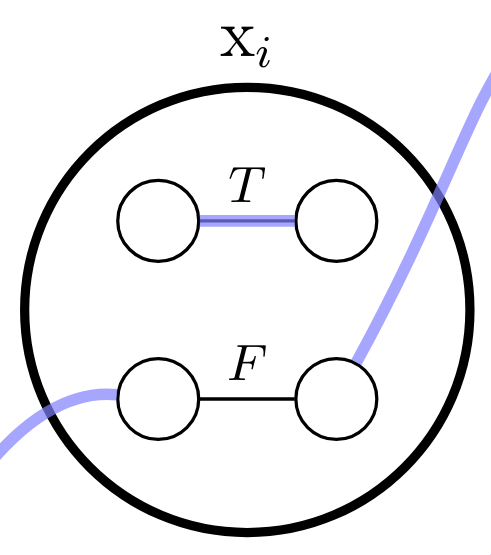
\includegraphics[height=4cm]{images/reduction/false.png}}
    \end{minipage}
\end{frame}

\begin{frame}{Clause Gadget}
    \centering
    $C_j = (x_a + x_b + x_c)$ and $C_k = (x_d + \bar x_e)$
    \bigbreak
    \begin{minipage}{\linewidth}
        \centering
        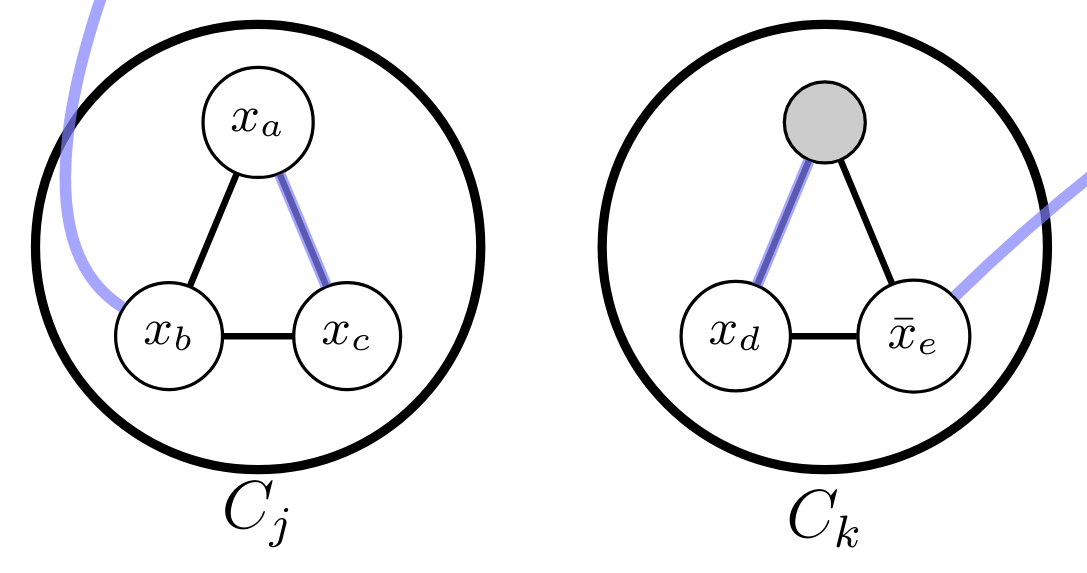
\includegraphics[height=4cm]{images/reduction/clause.png}
    \end{minipage}
\end{frame}

\begin{frame}{Complete Example}
    \centering
    $(\bar{x}_1 + x_3)(x_1 + x_2 + x_4)(x_1 + \bar{x}_4)(\bar{x}_2 + \bar{x}_3)(x_2 + x_3 + x_4)$ and $k=1$
    \begin{figure}
        \centering
        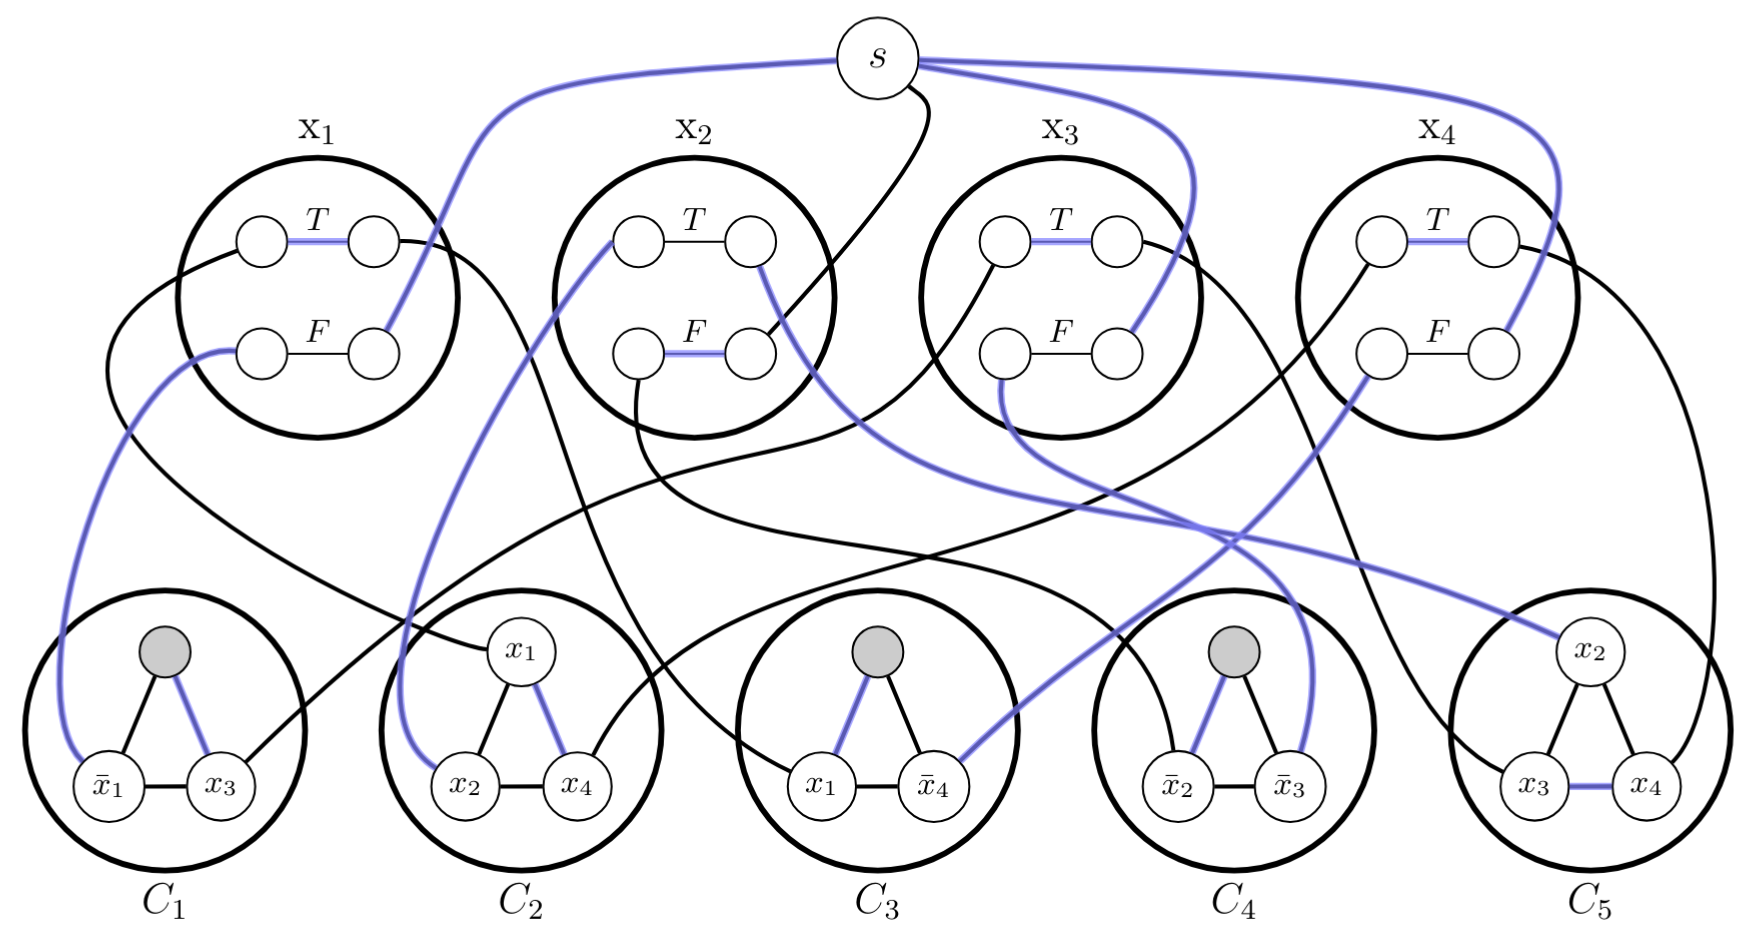
\includegraphics[width=0.9\textwidth]{images/reduction/full.png}
    \end{figure}
\end{frame}
